\section{Theorie}
\label{sec:Theorie}

\subsection{Aufbau und Funktionsweise eines Zählrohrs}

Das Geiger-Müller-Zählrohr besteht aus einem Kathodenzylinder mit dem Radius $r_k$ und einem entlang der Achse ausgerichtetem Anondendraht mit Radius $r_a$ (siehe Abb. \ref{fig:Rohr}).
\begin{figure}
  \centering
  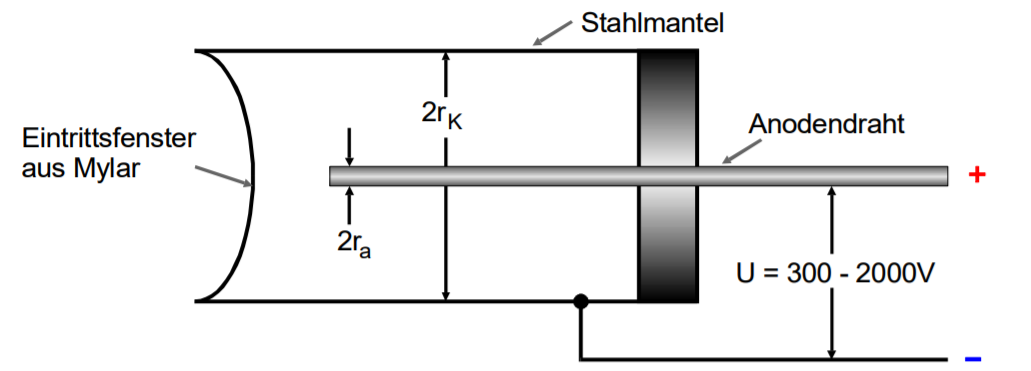
\includegraphics[height=3cm]{data/Rohr.png}
  \caption{Querschnitt eins Zählrohrs. \cite{V703}}
  \label{fig:Rohr}
\end{figure}
\FloatBarrier
Das Innere ist mit einem Gasgemisch gefüllt, das hauptsächlich mit der ionisierenden Strahlung wechselwirken soll.
Durch eine äußere Spannung $U$ wird ein radialsymmetrisches Feld erzeugt, das im Abstand $r$ folgende Feldstärke $E(r)$ besitzt:
\begin{equation}
  E(r) = \frac{U}{r \text{ln}(r_k/r_a)}
  \label{eqn:gl1s}
\end{equation}
Ein ionisierendes Teilchen, das in das Zählrohr eindringt, gibt seine Energie vollständig an die Gasatome ab und setzt dabei positive Ionen und Elektronen frei.
Die Prozesse, die nach dieser Primärionisation stattfinden, sind im wesentlichen von der angelegten Spannung abhängig.
Wie in Abbildung \ref{fig:Bereiche} zu sehen ist, kann die äußere Spannung in vier Bereiche mit verschiedenen Effekten unterteilt werden.
\begin{figure}
  \centering
  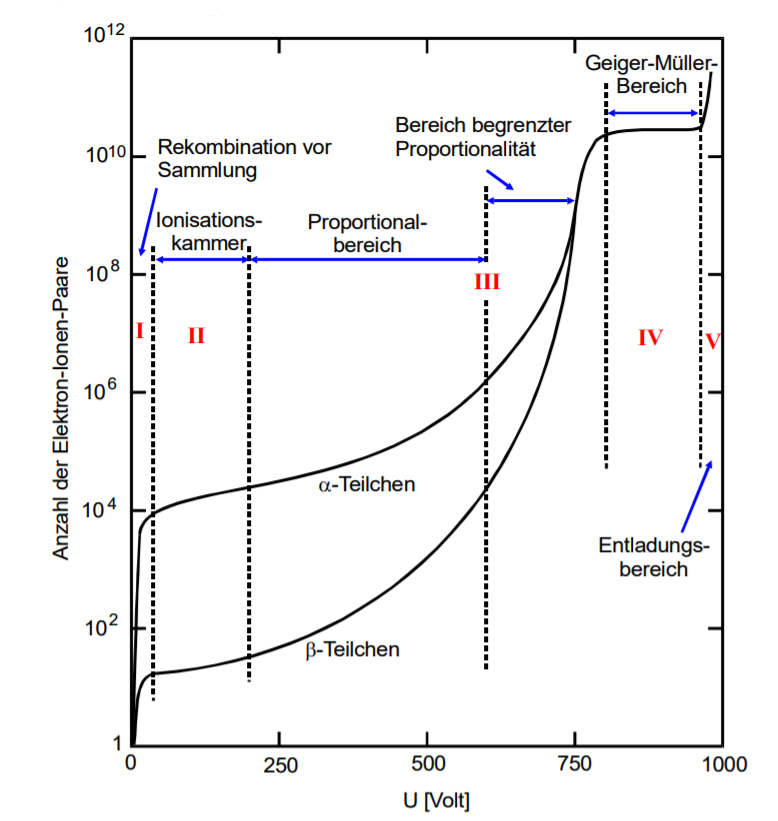
\includegraphics[height=9cm]{data/Bereiche.png}
  \caption{Anzahl der Elektronen-Ionenpaare in Abhängigkeit der äußeren Sapnnung $U$. \cite{V703}}
  \label{fig:Bereiche}
\end{figure}
Bei kleinen Spannungen im ersten Bereich, geht der größte Teil der freien Elektronen durch Rekombination verloren.
Wenn die Spannung groß genug wird (Bereich \RN{2}), ist das Auftreten der Rekombination verschwindend gering.
Quasi alle Elektronen erreichen den Anondendraht, der nun fließende Ionisationsstrom ist proportial zur Energie und der Intensität der ionisierenden Strahlung.
Ein Gerät, das mit diesen Spannungen arbeitet, wird Ionisationskammer genannt und funktioniert aufgrund des schwachen Ionisationsstroms nur bei hoher Strahlungsintensität.
Im dritten Spannungsbereich ist die Feldstärke so groß, dass die freigesetzten Elektronen selbst Gasatome ionisieren können.
Dieser Prozess wird als Stoßionisation bezeichnet und ionisieren die so freigesetzten Elektronen ebenfalls weitere Eletronen, nimmt die Anzahl der Elektronen wie eine Lawine zu.
Deshalb wird dieser Effekt als Townsend-Lawine bezeichnet.
Der so erzeugte Ladungsimpuls reicht aus, um gemessen werden zu können und ist immer noch proportial zur Strahlungsintensität und -energie, weswegen in diesem Fall vom Proportionalzählrohr gesprochen wird.
Bei weiterer Erhöhung der Spannung kommt es zu Anregungen der Gasatome, die dadurch UV-Strahlung emittieren.
Dieser Bereich \RN{4} ist der Auslösebereich und der Arbeitsbereich des Geiger-Müller-Zählrohrs.
Durch den Photoeffekt werden im ganzen Volumen des Zählrohrs weitere Elektronen-Lawinen ausgelöst, da sich die UV-Strahlung auch senkrecht zur Richtung des elektrischen Feldes ausbreiten kann.
Der Ionisationsstrom wird also unabhängig von der Strahlungsenergie und damit auch der Art der Strahlung, wie an dem Überlagern der Kurve der $\alpha$- und $\beta$-Strahlung in Abbildung \ref{fig:Bereiche} zu erkennen ist. \cite{V703}

\subsection{Totzeit, Erholungszeit und Nachentladungen}

Aufgrund ihrer deutlich größeren Masse der positiven Ionen befinden diese sich länger zwischen Kathode und Anode.
So entsteht ein radialsymmetrischer Ionenschlauch, der die Feldstärke um den Anondendraht herabsenkt.
Die Abschwächung ist zu Beginn so stark, dass keine Elektronen-Lawinen ausgelöst werden und somit keine ionisierenden Teilchen detektiert werden.
Dieser Zeitram wird als Totzeit $T$ bezeichnet.
Mit dem Abfließen der positiven Ionen ist eine Lawinenbildung und eine erneute Registrierung eines Ereignisses wieder möglich.
Aber erst nach der Erholungszeit $T_E$ kann der Ladungsimpuls wieder in voller Höhe gemessen werden, wenn alle Ionen neutralisiert werden.
Wenn die Ionen auf den Kathodenzylinder treffen, können diese Dank ihrer hohen Energie aus der Oberfläche Elektronen auslösen.
Diese Sekundärelektronen können selbst Elektronen-Lawinen und anschließende Ladungsimpulse hervorrufen.
Da die Zeitspanne dieser so genannten Nachentladungen größer als die Totzeit ist, können diese fälschlicherweise als Strahlungsereignis aufgefasst werden.
Deshalb sind Nachentladungen höchst unerwünscht und werden durch die Zugabe von Alkoholdämpfen unterdrückt.
Die durch die Strahlung ionisierten Edelgasatome treffen auf die Alkoholmoleküle, die aufgrund ihrer niedrigeren Ionisationsenergie ebenfalls ionisiert werden.
Die Alkoholmoleküle besitzen nicht genug Energie, um Elektronen auszulösen, wenn sie anstelle der Edelgasatome auf die Kathode treffen. \cite{V703}

\subsection{Charakteristik des Zählrohrs}

Die Charakteristik ist die Abhängigkeit der registrierten Teilchenzahl $N$ von der angelegten Spannung $U$ bei konstanter Strahlungsintensität.
Ein Schema der Charakteristik ist in Abbildung \ref{fig:Charakteristik} zu sehen.
\begin{figure}
  \centering
  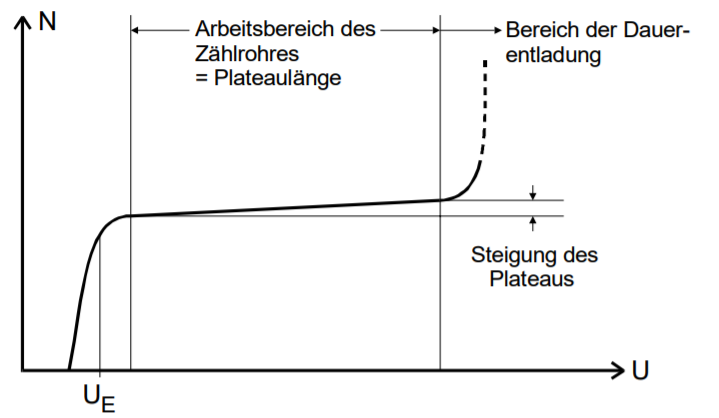
\includegraphics[height=6cm]{data/Charakteristik.png}
  \caption{Charakteristik eines Geiger-Müller-Zählrohrs. \cite{V703}}
  \label{fig:Charakteristik}
\end{figure}
Der Auslösebereich fängt ungefähr bei $U_E$ an und darauf folgt der der lineare Teil der Kurve, das Plateau.
Bei einem idealen Zählrohr ist die Plateausteigung gleich Null.
Da in der Realität trotz der Alkoholdämpfe Nachentladungen auftreten, weicht diese leicht von Null ab.
Nach dem Plateau ist die Spannung so groß, dass es im Zählrohr zu schädlichen Dauerentladungen kommt (siehe auch Abb. \ref{fig:Bereiche}). \cite{V703}
